\documentclass[10pt]{article}

\usepackage[T1]{fontenc}
\usepackage{amsmath}
\usepackage{newtxtext}
\usepackage{newtxmath}
\usepackage{microtype}
\usepackage[margin=1in]{geometry}
\usepackage{booktabs}
\usepackage{graphicx}
\usepackage{xcolor}
\usepackage[authoryear,round]{natbib}
\usepackage{algorithm}
\usepackage{algpseudocode}
\usepackage[colorlinks=true,linkcolor=blue!50!black,citecolor=blue!50!black,urlcolor=blue!50!black]{hyperref}
\usepackage[capitalise,noabbrev]{cleveref}

% Result-dependent text is marked in red and must be filled before release.
\newcommand{\placeholder}[1]{\textcolor{red}{[#1]}}

\newcommand{\PAL}{\mathcal{L}_{\mathrm{PAL}}}
\newcommand{\CE}{\mathcal{L}_{\mathrm{CE}}}
\newcommand{\sg}{\operatorname{sg}}

\title{A Synchronization Critic Improves\\Video-to-Audio Timing at Sampling Time}
\author{Samer Aslan\\Johns Hopkins University}
\date{}

\begin{document}
\maketitle

\begin{abstract}
Video-to-audio (V2A) generators usually produce the right kind of sound for a scene, but often at the wrong moment. We study how a synchronization critic can improve the timing of a codebook V2A generator (SpecVQGAN). The critic is a small audio-visual model, trained contrastively on real clips to find the offset between audio and video and then frozen. Its score, the Perceptual Alignment Loss (PAL), is the share of the critic's offset distribution that falls inside a window around zero offset, a simplified stand-in for the human audio-visual temporal binding window. We compare two ways to use PAL. As a differentiable training loss, passed to the transformer's logits through straight-through codebook decoding, PAL makes timing worse on FlashDot, a synthetic benchmark of flashing dots and tones with frame-exact labels. Two diagnostics suggest why: teacher-forced predictions inherit their alignment from the ground-truth prefix, so they look aligned without using the video, and optimizing free logits against the frozen critic reaches the score of real audio while the decoded audio stays poorly timed. As a reward on the generator's own free-running samples, the same critic helps: keeping the best of several samples improves timing on the FlashDot test split in every seed and on the open-domain VAS dataset. PAL-filtered self-training, which fine-tunes the generator on its own best-scored samples, does not keep this gain: it does no better than fine-tuning on randomly chosen samples, and it does not improve timing over the model it starts from. We also find that envelope lag recovers known delays exactly, while DTW distance tolerates time shifts by construction and is unsuited as a timing metric. In our experiments a synchronization critic improved the timing of a discrete-token V2A model only when it chose among samples at generation time. Code and FlashDot: \url{https://github.com/sameraslan/PerceptAlign}.
\end{abstract}

\section{Introduction}
\label{sec:intro}

People can predict from a silent video both what a hammer on a nail sounds like and when each impact happens. Video-to-audio (V2A) generation asks a model to do the same: produce a soundtrack that fits the frames of a silent clip, for uses such as Foley for film and sound for generated video. Codebook-transformer models \citep{iashin2021taming} and their successors usually get the kind of sound right. Timing is harder: a hammer clip can receive convincing hammer sounds whose impacts land between the visible strikes.

Part of the reason is the training objective. A codebook transformer is trained with cross-entropy over discrete spectrogram tokens, which has no notion of temporal distance: a token that would be correct two frames later scores the same as one that is wrong everywhere, so an onset placed slightly early costs about as much as one placed a second early.

Human perception handles timing with some tolerance. Light and sound from one event arrive at slightly different times, and observers still bind them into one event when the asynchrony falls inside the temporal binding window \citep{wallace2014construct}. The window is wider when audio lags than when it leads \citep{dixon1980detection,vanwassenhove2007temporal,vroomen2010perception}, varies between people \citep{stevenson2012individual}, and shifts after exposure to a constant lag \citep{fujisaki2004recalibration}. We take one design principle from this literature: a timing objective should accept small offsets around zero and penalize large ones, rather than treating every non-zero offset as equally wrong. Calling the loss ``perceptual'' is an analogy; we do not model the perceptual system.

Following the frozen sync-expert loss of Wav2Lip \citep{prajwal2020wav2lip} and the offset-distribution loss of \citet{niu2023synchronization}, we apply a frozen, contrastively pretrained synchronization critic as a training loss for open-domain video-to-audio generation, and make it differentiable for a discrete-token generator by decoding the generator's logits through the frozen codebook decoder with a straight-through estimator. We call the loss the Perceptual Alignment Loss (PAL). For each short segment of a clip, the critic compares audio and video embeddings at every offset in a small range and turns the comparisons into a distribution over offsets; PAL rewards the mass that falls inside a window around zero. The loss form is the self-synchronization loss of \citet{niu2023synchronization}. The changes are a soft window over near-zero offsets in place of their one-hot target, an optional asymmetric window, and computation per segment, so that a clip is aligned locally rather than on average.

Measuring timing also needs care: a metric that compares a generated spectrogram with the ground truth can be dominated by spectral content and barely move when the timing is off. We therefore test candidate metrics against known delays, and we build a benchmark where the correct timing is known exactly.

\paragraph{Contributions.}
\begin{itemize}
  \item \textbf{PAL}, a synchronization loss for codebook-based V2A generators: a binding-window target over offsets, computed per segment, applied through a frozen critic, with straight-through codebook decoding so that the loss reaches the transformer's logits (\cref{sec:method}).
  \item \textbf{FlashDot}, a synthetic benchmark of flashing dots and synchronous tones with frame-exact timing labels, in the SpecVQGAN data format (\cref{sec:data}).
  \item \textbf{A metric sensitivity check} measuring how candidate timing metrics respond to known delays (\cref{sec:res-metrics}).
  \item \textbf{Experiments} on FlashDot, training from scratch, and on VAS \citep{chen2020regnet}, fine-tuning the public SpecVQGAN transformer, with window ablations and a comparison against re-ranking samples with the same critic (\cref{sec:res-flashdot,sec:res-vas}).
\end{itemize}

\section{Related work}
\label{sec:related}

\paragraph{Video-to-audio generation.}
Early systems include example-based synthesis on Greatest Hits \citep{owens2016visually}, waveform generation on VEGAS \citep{zhou2018visual} and RegNet on VAS \citep{chen2020regnet}. SpecVQGAN \citep{iashin2021taming}, our base model, adapts VQGAN \citep{esser2021taming} to spectrograms and predicts codes from visual features with a transformer. Other systems improve alignment through architecture or visual features \citep{mei2024foleygen,wang2024frieren,viertola2025vaura,cheng2025mmaudio,mo2025foleyflow}, or condition on a timing signal predicted from video such as onsets, energy or a coarse layout \citep{comunita2024syncfusion,zhang2026foleycrafter,ton2025taro,jeong2025rewas,wang2024tiva}. Semantic conditioning without a timing mechanism is also common \citep{sheffer2023im2wav,wang2024v2amapper}.

\paragraph{Synchronization signals for V2A.}
Several systems use a synchronization model on whole outputs. CondFoley \citep{du2023conditional} re-ranks samples from a code model with a synchronization model at test time. Diff-Foley \citep{luo2023difffoley} guides diffusion sampling with an alignment classifier, and Seeing and Hearing \citep{xing2024seeing} steers pretrained generators with a frozen multimodal aligner. V2A-DPO \citep{chan2026v2adpo} and SyncDPO \citep{cheng2026syncdpo} post-train with preference pairs that reward synchronization. Our self-training is in the same family of sample-level rewards, with a binding-window critic as the reward and supervised fine-tuning on selected samples in place of a preference objective.

\paragraph{Synchronization models and losses.}
SyncNet \citep{chung2016outoftime} learned a two-stream embedding for lip sync. \citet{owens2018audio} learned audio-visual features by detecting shifted audio, the supervision our critic uses, and \citet{chung2019perfect} trained with a softmax over many candidate offsets, the form of our critic objective. Later models cover lips and voices \citep{kadandale2022vocalist,chen2024mtdvocalist}, localization \citep{afouras2020self,arandjelovic2018objects} and open-domain video \citep{iashin2022sparse,iashin2024synchformer}. Inside generators, Wav2Lip \citep{prajwal2020wav2lip} trains a face generator against a frozen sync expert, VCA-GAN \citep{kim2021vcagan} adds a contrastive synchronization term to lip-to-speech, \citet{niu2023synchronization} use the negative log probability of zero offset from a cross-correlation over offsets, and LatentSync \citep{li2024latentsync} carries SyncNet supervision into latent diffusion. These methods produce continuous outputs for lips and speech; we ask whether the same kind of loss transfers to a discrete-token sound-effect generator, and find that it does not.

\paragraph{Exposure bias, self-training and reward over-optimization.}
Teacher forcing conditions each prediction on the ground-truth prefix, so training never sees the model's own errors; scheduled sampling feeds model predictions back during training \citep{bengio2015scheduled}, and sequence-level training scores whole generated sequences \citep{ranzato2016sequence}. Training on a model's own filtered outputs appears in expert iteration \citep{anthony2017thinking} and in ReST \citep{gulcehre2023rest}, which alternate sampling from the current policy, filtering by a reward and fine-tuning on the kept samples; our self-training follows that loop with a synchronization critic as the filter. A learned reward that is optimized hard drifts away from the quantity it stands for \citep{gao2023scaling}; our free-logit attack measures the extreme case, with no generator between the optimizer and the critic.

\paragraph{Human audio-visual timing.}
Observers perceive auditory and visual signals as one event over a range of asynchronies, the temporal binding window \citep{wallace2014construct}. Audio lead is detected at smaller asynchronies than audio lag \citep{dixon1980detection}, and the window for audio-visual speech is wider on the audio-lag side \citep{vanwassenhove2007temporal,vroomen2010perception}. Its width differs across individuals \citep{stevenson2012individual}, and perceived simultaneity recalibrates after exposure to a constant lag \citep{fujisaki2004recalibration,takeshima2021visual}. We use these findings only to motivate the shape of the target over offsets.

\section{Method}
\label{sec:method}

\begin{figure}[t]
  \centering
  \fbox{\parbox[c][3.2cm][c]{0.9\linewidth}{\centering\placeholder{Figure 1: pipeline}}}
  \caption{Training pipeline. Stage 1: the critic embeds a real spectrogram (ground truth or its VQGAN reconstruction) and the clip's visual features and is trained so that zero offset wins the softmax over offsets. Stage 2: the critic and VQGAN decoder are frozen; a window of the transformer's logits is decoded with a straight-through estimator, scored by the critic, and PAL is added to the cross-entropy loss.}
  \label{fig:pipeline}
\end{figure}

\subsection{Base generator: SpecVQGAN}
\label{sec:specvqgan}

We follow the data geometry and models of SpecVQGAN \citep{iashin2021taming} (\cref{fig:pipeline}). Audio is an 80-bin log-mel spectrogram (22.05\,kHz, hop 256, 86.1 frames per second) of 848 frames, about 9.8\,s, with values in $[0,1]$. A VQGAN \citep{esser2021taming} encodes it into a $5 \times 53$ grid of codes from a codebook $E \in \mathbb{R}^{|V| \times 256}$, $|V| = 128$; one code column covers 16 mel frames. The transformer reads codes in column-major order (the five codes of a column, then the next column), so a sequence has $N = 265$ tokens. It is a GPT whose input starts with the clip's 212 visual feature frames (2048-dimensional, about 21.5 per second, so four per code column), projected by a $1 \times 1$ convolution and followed by the token embeddings. It is trained by teacher-forced cross-entropy, $\CE = -\frac{1}{N}\sum_{j} \log q_j(z_j)$ with $q_j = \operatorname{softmax}(\ell_j)$, where $z_j$ is the ground-truth code and $\ell_j \in \mathbb{R}^{|V|}$ the logits at position $j$. At test time codes are sampled autoregressively (top-$k$ with $k=100$, temperature 1) and decoded by the VQGAN decoder.

\subsection{Synchronization critic}
\label{sec:critic}

The critic has an audio encoder and a video encoder of the same structure: two blocks of a temporal one-dimensional convolution (kernel 5, 256 channels), group normalization (8 groups) and GELU, then a $1 \times 1$ convolution to 128 dimensions and L2 normalization at every frame. The audio input is the spectrogram mapped to $[-1,1]$ and average-pooled by four along time, which brings it to the 212-frame rate of the visual features. The design follows the local feature extractors of \citet{niu2023synchronization}, with group normalization in place of batch normalization and kernel 5 in both blocks (theirs uses 3 and 1). For a clip the critic gives unit-norm embeddings $a_1, \dots, a_T$ and $v_1, \dots, v_T$.

\subsection{Perceptual Alignment Loss}
\label{sec:pal}

For offsets $o \in \{-K, \dots, K\}$ (in video frames), PAL compares audio frame $i$ with video frame $i + o$, so a negative offset means the audio event comes after the visual one (audio late). Only the central frames $i \in [K, T-K)$ are used, so every offset compares the same number of real frames and none falls in the padding. The central region, of length $L = S \lfloor (T - 2K)/S \rfloor$, is split into $S$ equal consecutive segments $I_1, \dots, I_S$. For segment $s$,
\begin{equation}
  C_{s,o} = \frac{1}{|I_s|} \sum_{i \in I_s} \langle a_i, v_{i+o} \rangle, \qquad
  p_{s,o} = \frac{\exp(C_{s,o}/\tau)}{\sum_{o'=-K}^{K} \exp(C_{s,o'}/\tau)} .
  \label{eq:xcorr}
\end{equation}
The target is a window over offsets with weight one at zero,
\begin{equation}
  w_o = \exp\!\left(-\frac{o^2}{2\sigma_o^2}\right), \quad w_0 = 1, \quad
  \sigma_o = \begin{cases} \sigma_{\mathrm{late}} & o < 0 \ \text{(audio late)},\\ \sigma & o \geq 0 , \end{cases}
  \qquad W_s = \sum_{o=-K}^{K} w_o \, p_{s,o} \in (0, 1] .
  \label{eq:window}
\end{equation}
The symmetric window has $\sigma_{\mathrm{late}} = \sigma$; the asymmetric option sets $\sigma_{\mathrm{late}} > \sigma$, widening the window on the audio-late side in the direction of the human asymmetry. With $\sigma = 0$ the window is the indicator of zero offset. PAL averages the windowed mass over segments and takes the negative logarithm:
\begin{equation}
  \PAL = -\log\!\left(\frac{1}{S}\sum_{s=1}^{S} W_s\right).
  \label{eq:pal}
\end{equation}
With $\sigma = 0$ and $S = 1$, \cref{eq:pal} is $-\log p_{1,0}$, the self-synchronization loss of \citet{niu2023synchronization}. The window lets the generator put mass one or two frames from zero at a small cost, while mass at large offsets earns nothing. Segmentation makes the critic judge alignment over short stretches, so one well-aligned stretch cannot hide a badly aligned one behind a single clip-level score. The implementation also offers the reduction $-\frac{1}{S}\sum_s \log W_s$, which penalizes each badly aligned segment separately; stage 1 uses it.

\subsection{Stage 1: training the critic}
\label{sec:stage1}

The critic is trained on real clips with $\sigma = 0$, $K = 10$, $S = 8$, $\tau = 0.1$ and the per-segment log reduction, so the negatives are the other offsets of the same clip \citep{owens2018audio,chung2019perfect} and the objective is a cross-entropy over offsets with zero offset as the target in every segment. The audio input is the VQGAN reconstruction of the ground truth, since every spectrogram the critic sees in stage 2 comes out of the same decoder; with probability 0.3 per example it is the ground truth instead. The checkpoint with the lowest development loss is kept (\cref{tab:hparams}).

\subsection{Stage 2: training the generator with PAL}
\label{sec:stage2}

The critic and the VQGAN decoder are frozen; only the transformer, or its low-rank adapters (\cref{sec:models}), is trained. The critic needs a spectrogram, while the transformer outputs a distribution over codes. With $q_j = \operatorname{softmax}(\ell_j)$ from the teacher-forced cross-entropy pass, the decoded code vector is
\begin{equation}
  \hat e_j = \Bigl(\operatorname{onehot}\bigl(\arg\max_k q_{j,k}\bigr) + q_j - \sg(q_j)\Bigr)^{\!\top} E ,
  \label{eq:st}
\end{equation}
where $\sg$ stops the gradient \citeneeded{Bengio et al.\ 2013, straight-through estimator}. The forward value is the codebook entry of the most likely code, so the decoder only receives real codebook entries, and the backward pass uses the gradient of the expected code vector $q_j^{\top} E$. The code vectors are arranged back into the code grid and decoded by the frozen decoder into a spectrogram in $[-1, 1]$ that goes to the critic directly. (Soft decoding, which also uses $q_j^{\top} E$ in the forward pass, is an ablation.) Because the logits are teacher-forced, PAL scores the per-position most likely codes given the ground-truth prefix rather than a free-running sample.

Decoding all 53 columns and backpropagating through the decoder is expensive, so PAL uses a random window. At each step a start column $c_0$ is drawn uniformly, $c + 2m$ columns are decoded with $c = 12$ and margin $m = 1$, and the $16m$ mel frames at each end are discarded, since near the window's edges the decoder lacks the neighboring columns of a full decode. The remaining 192 mel frames are pooled by the critic to 48 frames and compared with the 48 visual feature frames starting at frame $4(c_0 + m)$. Stage 2 uses $K = 8$, $S = 4$, $\tau = 0.1$ and $\sigma = 1$: the central region of 32 frames gives four segments of about 0.37\,s, and offsets reach about $\pm 0.37$\,s. The decoder and critic run in half precision, with activation checkpointing in the decoder. PAL is computed on the first $B_{\mathrm{PAL}} = 4$ examples of each batch of 16, and the loss is
\begin{equation}
  \mathcal{L} = \CE + \beta \, \PAL ,
  \label{eq:total}
\end{equation}
with cross-entropy over the full batch and $\beta = \placeholder{value}$ chosen on the development split.

\section{Experimental setup}
\label{sec:setup}

\subsection{Datasets}
\label{sec:data}

\paragraph{FlashDot.}
FlashDot is a synthetic benchmark in which the correct timing is known exactly (example in \cref{fig:flashdot}). Each 10\,s clip shows a red dot on a white background during 1--6 ``on'' intervals of 0.15--1.5\,s and plays a 1\,kHz tone during exactly the same intervals; video runs at 21.5 frames per second, and clips are generated from a seed. Spectrograms follow the SpecVQGAN VAS pipeline, and visual features are the 2048-dimensional pooled outputs of an ImageNet-trained ResNet-50 \citep{he2016resnet}, one per frame. We generate 2000 clips, split 1600/200/200 into train, development and test.


\paragraph{VAS.}
VAS \citep{chen2020regnet} has eight classes (baby, cough, dog, drum, fireworks, gun, hammer, sneeze). We use the spectrograms and features released with SpecVQGAN \citep{iashin2021taming}: BN-Inception \citep{ioffe2015batch} RGB and optical-flow features, flow from denseflow \citep{wang2020denseflow}, concatenated to 2048 dimensions, 212 frames per clip. The test set is SpecVQGAN's \texttt{vas\_valid} list (768 clips). A class-stratified 5\% of \texttt{vas\_train} is held out as a development split (589 clips), and the remaining 11{,}184 clips are used for training.

\subsection{Models}
\label{sec:models}

On FlashDot we train a GPT with 6 layers, 6 heads and width 384 from scratch on codes from the public SpecVQGAN VAS codebook, which is not retrained (batch 8, 2000 steps unless stated). On VAS we start from the public SpecVQGAN VAS transformer (24 layers, 16 heads, width 1024). To fit training on a laptop GPU, its weights are frozen in half precision and only LoRA adapters \citep{hu2022lora} are trained, on the key, query, value and output projections and both MLP layers of every block (rank 16, $\alpha = 16$, initialized so that training starts from the public model). All training uses AdamW \citep{loshchilov2019adamw}. \Cref{tab:hparams} lists all hyperparameters.

\subsection{Metrics}
\label{sec:metrics}

Timing metrics compare a generated spectrogram with the ground-truth spectrogram of the same clip. The onset envelope is the spectral flux of the log-mel spectrogram (the sum over bins of positive frame-to-frame differences). \emph{Onset F1} matches generated and ground-truth onsets one to one within $\pm 100$\,ms \citep{raffel2014mireval}. \emph{Onset AP} ranks generated onsets by strength and counts a hit when one falls within $\pm 100$\,ms of an unmatched ground-truth onset, as in \citet{du2023conditional}. For the envelope metrics both envelopes are smoothed and mean-centred: \emph{envelope correlation} is their Pearson correlation at zero lag, and \emph{lag} is the shift within $\pm 1$\,s that maximizes their cross-correlation, reported as mean absolute value in ms and as the share of clips \emph{within one video frame} ($|\mathrm{lag}| \le 46.5$\,ms).

On FlashDot, \emph{tone F1} is the frame-level F1 between the ground-truth on/off label and a tone detector that thresholds the mean of the three mel bins with the largest on-minus-off difference. Bins and threshold are chosen on VQGAN reconstructions of training clips. Random codes score about 0.20.

Scoring a model with the critic it was selected against invites reward hacking, so \emph{held-out sync accuracy} uses a separate evaluation critic trained with the stage-1 recipe, a different seed and a different architecture (kernel 3, three blocks, width 384; on VAS its audio input is 8 band energies). It scores the whole clip ($S = 1$, $\sigma = 0$) over 21 offsets; we report the fraction of clips whose most likely offset is zero (tolerance 0) or within one frame of zero (tolerance 1). Chance is about $1/21$ and $3/21$. The critics are weak on VAS: development offset accuracy is 0.116 (0.288 within one frame) for the training critic and 0.124 (0.311) for the held-out critic. On FlashDot the training critic reaches 0.78 (0.81), limited by silent segments, which have no offset to find. On VAS we also report Melception FID and mean KL divergence (MKL) as in SpecVQGAN \citep{iashin2021taming}. The metric check (\cref{sec:res-metrics}) adds DTW distance on per-clip standardized mel frames \citep{salvador2007fastdtw} and mean absolute mel difference (mel L1).

\subsection{Protocol}
\label{sec:protocol}

All settings are chosen on the development split, and each final configuration is run on the test split once. The FlashDot loss experiments and the preliminary re-ranking result are single runs (seed 0) on the development split; they are diagnostic. Main FlashDot results use three seeds (0, 1, 2) on the test split and report the mean and standard deviation over seeds; VAS results use one seed, because each fine-tuning arm takes several hours on our hardware. Comparisons between two systems on the same clips use a paired bootstrap over clips (10{,}000 resamples) of the per-clip difference, computed separately for each seed and reported as a 95\% percentile interval and a two-sided $p$ value, checked against a paired sign-flip permutation test. Seeds are the unit of replication: we report each seed's comparison rather than pooling clips across seeds. The window width $\sigma = 1$ was fixed in advance as the default for test runs; the window comparison on the test split is exploratory and not corrected for multiple comparisons.

\section{Results}
\label{sec:results}

\subsection{Which metrics respond to known delays}
\label{sec:res-metrics}

A timing metric should worsen steadily as a known delay grows and should rank a clip with the right kind of sound but unrelated timing as badly aligned. We delay each of 200 FlashDot development spectrograms by 2 to 64 mel frames (23 to 743\,ms), filling the start with the clip's quietest frame, and compare it with the original; as a second reference we compare each clip with a different clip (\cref{fig:sensitivity}; values in \cref{tab:sensitivity}).


\begin{figure}[t]
  \centering
  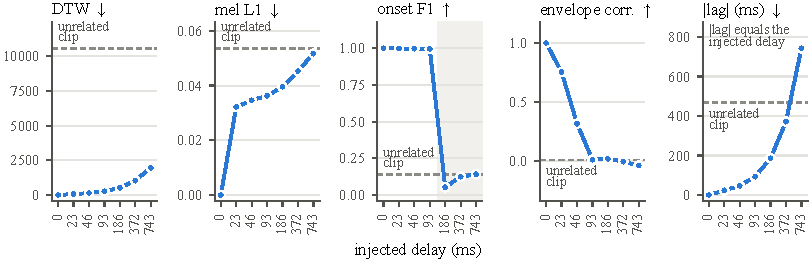
\includegraphics[width=\linewidth]{figures/metric_sensitivity.pdf}
  \caption{Metric response to injected delays on FlashDot (development, 200 clips). Dashed lines: an unrelated clip. Only $|$lag$|$ grows in proportion to the delay; DTW and mel L1 rank every delay as closer to the truth than an unrelated clip.}
  \label{fig:sensitivity}
\end{figure}

On FlashDot, where each delay is a pure shift of identical audio, the envelope lag recovers the injected delay exactly. Onset F1 is flat up to 93\,ms, inside its tolerance, and drops to the level of an unrelated clip (about 0.14) or below from 186\,ms. Envelope correlation falls from 0.75 at 23\,ms to about zero by 93\,ms, so it cannot tell 100\,ms from a second. DTW grows with delay, from 69 at 23\,ms to 1968 at 743\,ms, but an unrelated clip scores 10582: a large delay looks five times closer to the truth than a clip with different content. This is expected, since DTW tolerates time shifts by construction, and it makes DTW unsuited as a timing metric. Mel L1 jumps at the smallest delay and then barely separates a 743\,ms delay (0.052) from an unrelated clip (0.054). We therefore use $|$lag$|$, within-one-frame, onset F1 and, on FlashDot, tone F1 as timing metrics, and leave DTW out. These delays are exact shifts of identical audio, so the check shows how each metric responds to a pure delay and does not establish how well it tracks timing errors in generated audio.

\subsection{PAL as a training loss does not improve timing}
\label{sec:res-loss}

% Generated by perceptalign/paper_tables.py; do not edit by hand (sources: paper/generated/sources.md).
\providecommand{\std}[1]{\,{\scriptsize$\pm$#1}}
\begin{table}[t]
  \centering
  \caption{FlashDot. Top: references. Middle: PAL as a loss and the CE baselines, trained from scratch (development split, 2000 steps unless stated). Bottom: PAL as a reward. Sync acc.\ is the held-out critic at tolerance 1 (chance $\approx 0.14$); within 1 frame is the share of clips with $|$lag$|$ within one video frame. Mean $\pm$ std over three training seeds; $^{\dagger}$\,single training seed. Best of 8 on the development split uses training seed 0.}
  \label{tab:flashdot}
  \small
  \begin{tabular}{llcccc}
    \toprule
    Model & Split & Tone F1 $\uparrow$ & $|$Lag$|$ (ms) $\downarrow$ & Within 1 frame $\uparrow$ & Sync acc.\ $\uparrow$ \\
    \midrule
    VQGAN reconstruction                                 & dev  & 0.970 & 2.7 & 1.000 & 1.000 \\
    VQGAN reconstruction                                 & test & 0.971 & 4.9 & 0.995 & 1.000 \\
    \midrule
    CE (teacher forcing)                                 & dev  & 0.414\std{0.007} & 410\std{14} & 0.108\std{0.020} & 0.200\std{0.030} \\
    CE, corrupted prefix ($p_{\mathrm{keep}} = 0.5$)     & dev  & 0.501\std{0.028} & 317\std{15} & 0.190\std{0.017} & 0.267\std{0.033} \\
    CE + PAL, teacher-forced (3000 steps)                & dev  & 0.315\std{0.016} & 485\std{26} & 0.050\std{0.015} & 0.112\std{0.033} \\
    CE + PAL, half-corrupted PAL prefix                  & dev  & 0.255\std{0.024} & 502\std{24} & 0.055\std{0.020} & 0.117\std{0.006} \\
    CE + PAL, fully corrupted PAL prefix$^{\dagger}$     & dev  & 0.279 & 491 & 0.060 & 0.125 \\
    \midrule
    CE, corrupted prefix, best of 8$^{\dagger}$          & dev  & 0.535 & 228 & 0.480 & 0.645 \\
    \midrule
    CE, corrupted prefix                                 & test & 0.498\std{0.014} & 340\std{12} & 0.198\std{0.016} & 0.233\std{0.016} \\
    \quad best of 8                                      & test & 0.567\std{0.027} & 239\std{14} & 0.422\std{0.026} & 0.705\std{0.031} \\
    \quad self-training, random selection                & test & 0.449\std{0.012} & 384\std{21} & 0.128\std{0.033} & 0.178\std{0.033} \\
    \quad self-training, PAL selection                   & test & 0.458\std{0.029} & 359\std{24} & 0.133\std{0.010} & 0.185\std{0.020} \\
    \bottomrule
  \end{tabular}
\end{table}


On FlashDot, every way of adding PAL to the loss lowers timing quality (\cref{tab:flashdot}, middle; means over three training seeds on the development split, except for the fully corrupted row, which is one seed). With teacher-forced logits, tone F1 falls from 0.414 to 0.315 and held-out sync accuracy (tolerance 1) from 0.200 to 0.112, below chance (about 0.14), even with 1000 more training steps. Computing PAL from a half or fully corrupted prefix, so that the video is the only source of timing, does no better (tone F1 0.255 and 0.279). Corrupting the prefix of the cross-entropy pass alone, with no critic, helps instead: tone F1 0.501, $|$lag$|$ 317\,ms. The two diagnostics of \cref{sec:diagnostics} are consistent with the shortcut account below. They do not exclude other causes of the drop, such as the single loss weight ($\beta = 1$) or interference between the two gradients.

\paragraph{Exposure bias.}
The CE model does use the video under teacher forcing: over the 200 development clips, and as a mean over three training seeds, development cross-entropy is 1.54 with each clip's own visual features and 1.89 with another clip's. With a fully corrupted prefix it is 4.51 against 4.66, close to the uniform level of 4.85, so the video alone tells the model little about which code comes next. This suggests that teacher-forced predictions inherit their timing from the aligned prefix and look aligned to the critic whatever the model does with the video, while the model's free-running samples have low timing accuracy (held-out sync accuracy 0.200 at tolerance 1, against a chance level of about 0.14). A PAL gradient on teacher-forced logits would then reward copying the prefix, which the model already does.

\paragraph{The critic can be exploited.}
Corrupting the PAL prefix removes the shortcut through the prefix but opens another one. In the free-logit attack (\cref{fig:attack}), optimizing logits directly against the mel critic reaches a PAL of 0.98, about that of the ground-truth codes (0.95; random codes 2.12). The decoded spectrograms are broadband texture with tone F1 0.28, barely above random codes (0.20) and far from the ground truth (0.98). Critics that see only 8, 4 or 1 band energies are fooled the same way. Coarser critics do align energy changes better at the optimum, with $|$lag$|$ of 151\,ms (mel), 147\,ms (8 bands), 48\,ms (4 bands) and 15\,ms (1 band) against 644\,ms for random codes, but none of them produces the tone: tone F1 at the optimum is 0.28, 0.28, 0.11 and 0.05. A critic trained only on real audio has not seen spectrograms like these, which is a likely reason it scores them as aligned.

\begin{figure}[t]
  \centering
  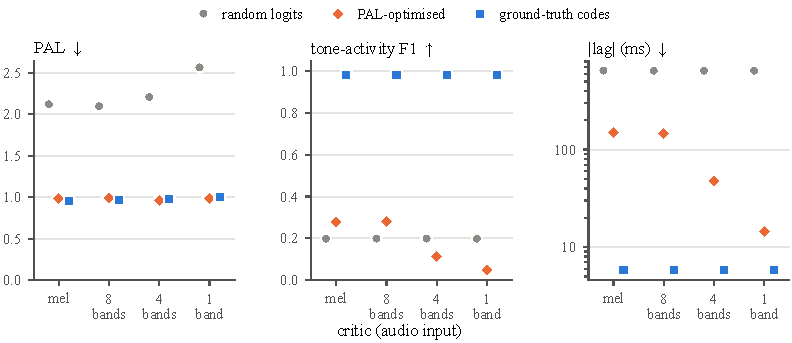
\includegraphics[width=\linewidth]{figures/critic_attack.pdf}
  \caption{Free-logit attack on four FlashDot critics (eight development clips). Optimizing logits against PAL (orange) reaches the PAL of the ground-truth codes (blue) for every critic, while tone F1 stays far below the ground truth (0.98): 0.28 for the mel and 8-band critics against 0.20 for random codes (grey), and lower for the 4-band and 1-band critics. Coarser critics bring the envelope lag down, but none recovers the tone.}
  \label{fig:attack}
\end{figure}

\subsection{PAL as a reward on samples}
\label{sec:res-reward}

Used to choose among the generator's own samples, the same critic helps. Keeping the best of eight free-running samples from the corruption-trained CE model (candidates scored with $\sigma = 0$) raises tone F1 from 0.499 to 0.535, the share of clips within one video frame from 0.17 to 0.48, and held-out sync accuracy (tolerance 1) from 0.245 to 0.645 on the FlashDot development split (training seed 0) (\cref{tab:flashdot}). The tone F1 gain is modest; the larger held-out gain partly reflects that the two critics share features and model family. \Cref{fig:fd-samples} shows one development clip: the clip whose $|$lag$|$ gain from re-ranking is the median over clips, so it shows a typical case rather than the best one.

\begin{figure}[t]
  \centering
  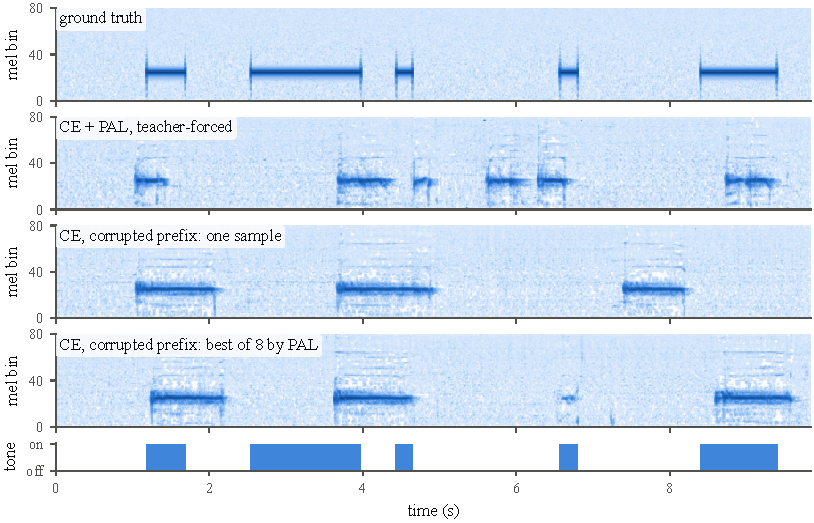
\includegraphics[width=\linewidth]{figures/flashdot_samples.pdf}
  \caption{One FlashDot development clip (the clip with the median $|$lag$|$ gain from best-of-8 re-ranking). The bottom row marks when the tone is on. The model trained with PAL as a loss (teacher-forced) adds tones that are not in the video; the corruption-trained CE model misses some tones; keeping the best of eight of its samples by PAL matches more of the tones (tone F1 0.57 on this clip, against 0.33 for the single sample), though its lag is still large (790\,ms against 859\,ms).}
  \label{fig:fd-samples}
\end{figure}

On the FlashDot test split, over three generator seeds and with candidates scored at $\sigma = 1$ (the setting used for VAS and for self-training), best-of-8 re-ranking raises tone F1 from 0.498 to 0.567, the share of clips within one frame from 0.20 to 0.42, and held-out sync accuracy (tolerance 1) from 0.23 to 0.71 (means over seeds). Seeds are the unit of replication, so we report each seed. Against one sample, best of 8 raises tone F1 by 0.054 ($p = 0.001$), 0.084 and 0.068 (both $p < 0.001$) and the share of clips within one frame by 0.205, 0.195 and 0.270 (all $p < 0.001$); the sign is the same in every seed. The oracle that keeps the candidate with the best true tone F1 reaches only 0.39 held-out sync accuracy against 0.71 for PAL selection (\cref{tab:window}), so the held-out score partly measures agreement with the selecting critic; tone F1 and the within-one-frame share are the primary timing measures.

Self-training does not keep this gain. After two rounds (400 clips per round, eight candidates, 300 steps), mean tone F1 falls to 0.458 with PAL selection and 0.449 with random selection, below the 0.498 of the starting model, and the share of clips within one frame falls from 0.20 to 0.13 with either rule. Per seed (0, 1, 2), the change in tone F1 against the starting model is $-0.010$ ($p = 0.47$), $-0.052$ and $-0.059$ (both $p < 0.001$) with PAL selection and $-0.043$ ($p = 0.002$), $-0.056$ and $-0.050$ (both $p < 0.001$) with random selection. PAL minus random selection is $+0.033$ ($p = 0.01$), $+0.004$ ($p = 0.75$) and $-0.008$ ($p = 0.54$) in tone F1, so the selection rule does not matter consistently. Because fine-tuning on the model's own samples lowered tone F1 with either selection rule, the FlashDot self-training arms say little about the critic's choice; the ground-truth-only control exists only on VAS.

% Generated by perceptalign/paper_tables.py; do not edit by hand (sources: paper/generated/sources.md).
\providecommand{\stackstd}[2]{\begin{tabular}[t]{@{}c@{}}#1\\[-2pt]{\scriptsize #2}\end{tabular}}
\begin{table}[t]
  \centering
  \caption{VAS test results (768 clips of the SpecVQGAN \texttt{vas\_valid} list), one sample per clip unless stated. Sync acc.\ is the held-out critic at tolerance 0 / 1 (chance $\approx 0.05$ / $0.14$). On.: onset; Env.: envelope correlation; $|$Lag$|$ in ms; 1 fr.: share of clips with $|$lag$|$ within one video frame. Fine-tuned rows train LoRA adapters with the same budget.}
  \label{tab:vas}
  \small
  \setlength{\tabcolsep}{3.2pt}
  \begin{tabular}{lcccccccc}
    \toprule
    Model & On.\ F1 $\uparrow$ & On.\ AP $\uparrow$ & Env.\ $\uparrow$ & $|$Lag$|$ $\downarrow$ & 1 fr.\ $\uparrow$ & Sync acc.\ $\uparrow$ & FID $\downarrow$ & MKL $\downarrow$ \\
    \midrule
    Ground truth                 & -- & -- & -- & -- & -- & 0.285 / 0.536 & -- & -- \\
    VQGAN reconstruction         & 0.813 & 0.778 & 0.918 & 0.2 & 100\% & 0.277 / 0.518 & 6.0 & 1.03 \\
    \midrule
    Pretrained SpecVQGAN         & 0.368 & 0.206 & 0.003 & 502 & 5.6\% & 0.061 / 0.167 & 27.8 & 5.81 \\
    \quad best of 4              & 0.376 & 0.215 & 0.015 & 456 & 6.6\% & 0.151 / 0.375 & 26.7 & 5.92 \\
    \quad GT-only fine-tune      & \placeholder{} & \placeholder{} & \placeholder{} & \placeholder{} & \placeholder{} & \placeholder{} / \placeholder{} & \placeholder{} & \placeholder{} \\
    \quad self-train, random     & \placeholder{} & \placeholder{} & \placeholder{} & \placeholder{} & \placeholder{} & \placeholder{} / \placeholder{} & \placeholder{} & \placeholder{} \\
    \quad self-train, PAL        & \placeholder{} & \placeholder{} & \placeholder{} & \placeholder{} & \placeholder{} & \placeholder{} / \placeholder{} & \placeholder{} & \placeholder{} \\
    \bottomrule
  \end{tabular}
\end{table}


On VAS (\cref{tab:vas}), the VQGAN reconstruction reaches FID 6.0 and MKL 1.03, matching the published codebook numbers (6.0 and 1.0), which checks our port of the evaluation. The pretrained SpecVQGAN transformer (top-$k$ 100, one sample per clip) gives FID 27.8 and MKL 5.81 (published 25.4 and 5.9). Its timing is close to chance: envelope correlation 0.003, $|$lag$|$ 502\,ms, 5.6\% of clips within one frame, and held-out sync accuracy at tolerance 0 / 1 of 0.061 / 0.167, against chance levels of about 0.05 / 0.14. The ground truth itself reaches only 0.285 / 0.536 (tolerance 0 / 1) under the held-out critic, which bounds what that metric can show. 

Keeping the best of four samples per clip by PAL improves the timing measures that follow the envelope: $|$lag$|$ falls by 46\,ms (95\% interval 16 to 74\,ms, $p = 0.002$, paired bootstrap over the 768 clips), envelope correlation rises from 0.003 to 0.015 ($p < 0.001$) and held-out sync accuracy at tolerance 1 from 0.167 to 0.375, at four times the sampling cost. Onset F1 ($+0.008$, $p = 0.10$) does not change significantly, and the share of clips within one frame stays at 5.6 to 6.6\% ($p = 0.41$), and FID and MKL stay close to the single-sample values. The held-out gain is the largest, and it is the one most open to shared bias between the two critics (\cref{sec:limitations}).

Self-training does not carry this gain into the generator. With the same LoRA budget (two rounds of 256 clips, four candidates, 150 steps each), self-training with PAL selection, self-training with random selection and fine-tuning on ground truth alone give the same timing: no two of the three differ significantly on any timing measure (all $p > 0.1$). For PAL against random selection, onset F1 differs by $+0.003$ ($p = 0.50$), $|$lag$|$ by $+22$\,ms ($p = 0.13$) and sync accuracy at tolerance 1 by $+0.001$ ($p = 0.98$). All three lower onset F1 by about 0.02 against the pretrained model ($p < 0.001$), and only random selection lowers $|$lag$|$ significantly ($-35$\,ms, $p = 0.01$). All three also lower FID, and ground-truth-only fine-tuning lowers it most (20.4, against 24.1 with PAL selection and 25.1 with random selection). On VAS this suggests that the FID gain comes from fine-tuning on in-domain audio (FID values are single runs), and at this budget PAL selection adds nothing measurable to timing or quality.

% Generated by perceptalign/paper_tables.py; do not edit by hand (sources: paper/generated/sources.md).
\providecommand{\std}[1]{\,{\scriptsize$\pm$#1}}
\begin{table}[t]
  \centering
  \caption{Candidate selection on the test split: every row chooses among the same 8 free-running samples per clip. FlashDot: corruption-trained CE generator, \placeholder{} clips, mean $\pm$ std over \placeholder{} generator seeds. VAS: pretrained SpecVQGAN, \placeholder{} clips, one run. $\sigma$: width of the binding window on the audio-early side, $\sigma_{\mathrm{late}}$ on the audio-late side (\cref{eq:window}). Sync: held-out critic at tolerance 1. The oracle keeps the candidate with the best true tone F1 (FlashDot) or smallest $|$lag$|$ (VAS).}
  \label{tab:window}
  \small
  \setlength{\tabcolsep}{3.2pt}
  \begin{tabular}{lccccccc}
    \toprule
    & \multicolumn{3}{c}{FlashDot} & \multicolumn{4}{c}{VAS} \\
    \cmidrule(lr){2-4} \cmidrule(lr){5-8}
    Selection & Tone F1 $\uparrow$ & 1 fr.\ $\uparrow$ & Sync $\uparrow$ & 1 fr.\ $\uparrow$ & $|$Lag$|$ $\downarrow$ & Sync $\uparrow$ & FID $\downarrow$ \\
    \midrule
    One sample                                           & \placeholder{} & \placeholder{} & \placeholder{} & \placeholder{} & \placeholder{} & \placeholder{} & \placeholder{} \\
    Best of 8, $\sigma = 0$                              & \placeholder{} & \placeholder{} & \placeholder{} & \placeholder{} & \placeholder{} & \placeholder{} & \placeholder{} \\
    Best of 8, $\sigma = 0.5$                            & \placeholder{} & \placeholder{} & \placeholder{} & \placeholder{} & \placeholder{} & \placeholder{} & \placeholder{} \\
    Best of 8, $\sigma = 1$                              & \placeholder{} & \placeholder{} & \placeholder{} & \placeholder{} & \placeholder{} & \placeholder{} & \placeholder{} \\
    Best of 8, $\sigma = 2$                              & \placeholder{} & \placeholder{} & \placeholder{} & \placeholder{} & \placeholder{} & \placeholder{} & \placeholder{} \\
    Best of 8, $\sigma = 0.5$, $\sigma_{\mathrm{late}} = 2$ & \placeholder{} & \placeholder{} & \placeholder{} & \placeholder{} & \placeholder{} & \placeholder{} & \placeholder{} \\
    Best of 8, $\sigma = 2$, $\sigma_{\mathrm{late}} = 0.5$ & \placeholder{} & \placeholder{} & \placeholder{} & \placeholder{} & \placeholder{} & \placeholder{} & \placeholder{} \\
    \midrule
    Oracle (upper bound)                                 & \placeholder{} & \placeholder{} & \placeholder{} & \placeholder{} & \placeholder{} & \placeholder{} & \placeholder{} \\
    \bottomrule
  \end{tabular}
\end{table}


\paragraph{Binding window.} \Cref{tab:window} scores the same eight candidates per clip under different windows. Every window improves on one sample. Tone F1 barely depends on the window (0.551 to 0.572 on FlashDot), while the other measures trade off: the within-one-frame share ranges from 0.370 to 0.463 and held-out sync accuracy from 0.590 to 0.705. On FlashDot the narrowest window ($\sigma = 0$, exact zero offset) puts more clips within one frame than $\sigma = 1$ in all three seeds (0.463 against 0.422 on average), but the difference is significant only in seed 0 ($p = 0.01$; $p = 0.36$ and $0.40$ in the others). In turn, $\sigma = 1$ gives higher held-out sync accuracy at tolerance 1, the tolerance that window matches, in all three seeds (0.705 against 0.590, $p < 0.001$ in each) and higher onset F1 in all three ($p \le 0.014$). On VAS (one run, 256 clips), $\sigma = 0$ and $\sigma = 1$ do not differ significantly on any measure. Neither asymmetric window gives a consistent gain over the symmetric $\sigma = 1$ window, and the window with a wide audio-late side ($\sigma = 0.5$, $\sigma_{\mathrm{late}} = 2$) lowers held-out sync accuracy relative to $\sigma = 1$ on FlashDot in all three seeds ($p \le 0.009$) and on VAS ($-0.066$, $p = 0.003$). The oracle rows show how far any PAL choice is from the best available candidate: on VAS, choosing by true lag puts 40\% of clips within one frame, against 7 to 9\% for every PAL window.

\section{Discussion}
\label{sec:discussion}

The same frozen critic hurts timing as a loss and helps as a selector at sampling time, and the two diagnostics are consistent with one account of the difference. A differentiable loss scores whatever the gradient path produces: under teacher forcing that is a prediction already aligned by its prefix, and with the prefix removed it is a point the generator can move toward freely, including spectrograms outside anything the critic was trained on. A reward on free-running samples scores only what the generator actually produces, so the critic works inside the region where its ranking means something. That ranking did not carry over into the generator's weights: fine-tuning on the critic's choices matched fine-tuning on random choices on both datasets, and on FlashDot both fell below the starting model. The gain from selection is specific to each clip and its video, and two short rounds of cross-entropy on a few hundred chosen samples did not teach the generator to make such choices itself; larger budgets or a training signal that compares candidates directly may behave differently. This matches what is known about optimizing learned rewards \citep{gao2023scaling}: the less freely the optimizer can move against the reward model, the more the reward keeps its meaning. For similar setups, we suggest running the wrong-video probe and the free-logit attack before training against a critic, and using the critic to select samples at generation time. Our results give no support to the perceptual motivation for the window: no window is best on every measure, and the asymmetric windows that follow the human tolerance for late audio bring no gain. We keep the window as a parameter of PAL rather than as a claim about perception.

\section{Limitations}
\label{sec:limitations}

\begin{itemize}
  \item \textbf{Base model.} SpecVQGAN is far from current V2A systems such as MMAudio \citep{cheng2025mmaudio}. Our results show whether PAL changes a codebook transformer's timing; they do not show that it would help a current flow or diffusion model, and we make no state-of-the-art comparison.
  \item \textbf{Compute.} All training ran on one laptop GPU, so on VAS we fine-tune low-rank adapters rather than the full transformer, compute PAL on a 12-column window of four examples per batch, and train for \placeholder{steps}. Larger budgets could change the size of the effect in either direction.
  \item \textbf{Feature-based critic and evaluation.} The critic sees precomputed visual features at about 21.5 frames per second, so one offset step is about 46\,ms and finer errors are invisible to it. The held-out critic uses the same features and model family, so it is not fully independent of the training critic. \placeholder{Add a Synchformer-based score \citep{iashin2024synchformer} if computed, or say it was not.}
  \item \textbf{Teacher-forced loss.} PAL scores the most likely codes under teacher forcing, which can differ from free-running samples.
  \item \textbf{Binding window.} The Gaussian window, symmetric or wider on the audio-late side, simplifies a human window whose width and shape vary with stimulus, task and observer \citep{stevenson2012individual,takeshima2021visual}; it is not fitted to human data.
\end{itemize}


\bibliographystyle{plainnat}
\bibliography{refs}

\appendix
\section{Relation to an earlier draft}
\label{app:earlier}

An unpublished 2023 draft of this work reported results for an earlier implementation of the alignment loss. In that implementation the loss could not influence the generator: the predicted spectrogram was decoded from the argmax of the transformer's logits inside a function that ran without gradient tracking, so no gradient reached the transformer, and the only parameters the loss touched, those of its two feature extractors, were not in the optimizer. All numbers in that draft are superseded by this paper. The experiments reported here were rerun with a new implementation in which the gradient does reach the transformer (\cref{sec:pal-loss}); with that path in place, the loss the draft intended does not improve timing (\cref{sec:res-loss}).

\section{FlashDot example and metric check values}
\label{app:extra}

\begin{figure}[h]
  \centering
  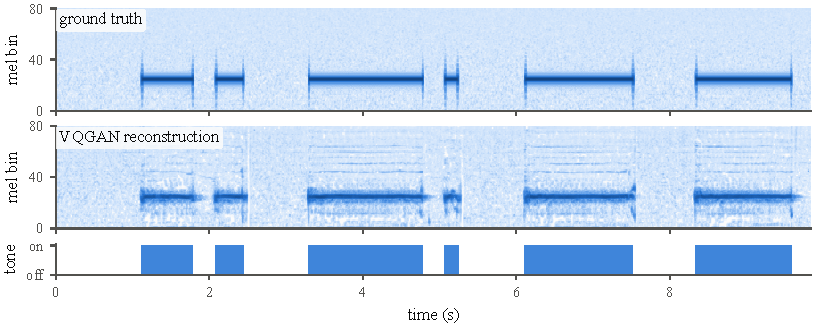
\includegraphics[width=0.85\linewidth]{figures/flashdot_example.pdf}
  \caption{A FlashDot clip: ground-truth spectrogram, its VQGAN reconstruction with the public VAS codebook, and the tone label. The reconstruction keeps the timing (tone F1 0.970 over the development split) and adds codebook texture, so it bounds what any code model with this decoder can reach.}
  \label{fig:flashdot}
\end{figure}

\begin{table}[h]
  \centering
  \caption{Response of candidate metrics to known delays, mean over 200 FlashDot development clips. Arrows give the direction of a better score.}
  \label{tab:sensitivity}
  \small
  \begin{tabular}{lccccc}
    \toprule
    Comparison & DTW $\downarrow$ & Mel L1 $\downarrow$ & Onset F1 $\uparrow$ & Env.\ corr.\ $\uparrow$ & $|$Lag$|$ (ms) $\downarrow$ \\
    \midrule
    Delay 0\,ms   & 0     & 0.000 & 1.00 & 1.00  & 0 \\
    Delay 23\,ms  & 69    & 0.032 & 1.00 & 0.75  & 23 \\
    Delay 46\,ms  & 138   & 0.035 & 1.00 & 0.32  & 46 \\
    Delay 93\,ms  & 271   & 0.036 & 1.00 & 0.01  & 93 \\
    Delay 186\,ms & 527   & 0.040 & 0.05 & 0.02  & 186 \\
    Delay 372\,ms & 1034  & 0.045 & 0.13 & $-0.01$ & 372 \\
    Delay 743\,ms & 1968  & 0.052 & 0.14 & $-0.04$ & 743 \\
    \midrule
    Other clip    & 10582 & 0.054 & 0.14 & 0.01  & 470 \\
    \bottomrule
  \end{tabular}
\end{table}

\clearpage
\section{Hyperparameters}
\label{app:hparams}

\begin{table}[h]
  \centering
  \caption{Hyperparameters. Values are those of the reported runs; red entries are not yet fixed.}
  \label{tab:hparams}
  \small
  \begin{tabular}{llc}
    \toprule
    Component & Setting & Value \\
    \midrule
    Training critic & encoder blocks / kernel / channels & 2 / 5 / 256 \\
           & embedding dimension, normalization & 128, L2 per frame \\
           & group norm groups, mel pooling & 8, $\times 4$ \\
    Held-out critic & blocks / kernel / channels, seed & 3 / 3 / 384, 1 \\
           & audio input (FlashDot / VAS) & mel / 8 bands \\
    \midrule
    Stage 1 & $K$, $\tau$, $\sigma$ & 10, 0.1, 0 \\
            & $S$ (FlashDot / VAS) & 4 / 8 \\
            & reduction & $-\frac{1}{S}\sum_s \log W_s$ \\
            & probability of ground-truth audio & 0.3 \\
            & optimizer & AdamW, lr $10^{-3}$, wd $10^{-4}$ \\
            & steps (FlashDot / VAS), batch & 2000 / 3000, 32 \\
            & selection & lowest dev loss \\
    \midrule
    PAL as a loss & $K$, $S$, $\tau$, $\sigma$ & 8, 4, 0.1, 1 \\
    (FlashDot) & reduction & $-\log \frac{1}{S}\sum_s W_s$ \\
            & decoding & straight-through \\
            & window columns $c$, margin $m$ & 12, 1 \\
            & examples with PAL per batch & 4 of 8 \\
            & PAL weight $\beta$ & 1 \\
            & $p_{\mathrm{keep}}$ (CE pass), $p^{\mathrm{PAL}}_{\mathrm{keep}}$ & $\{1, 0.5\}$, $\{1, 0.5, 0\}$ \\
            & optimizer & AdamW, lr $3 \times 10^{-4}$, $\beta = (0.9, 0.95)$, wd 0.01 \\
            & schedule, gradient clipping & 200 warm-up steps, cosine decay; 1.0 \\
            & steps, batch & 2000 (3000 teacher-forced PAL), 8 \\
    \midrule
    FlashDot GPT & layers / width / heads & 6 / 384 / 6 \\
    \midrule
    Self-training & rounds, steps per round & 2, 300 (FlashDot) / 150 (VAS) \\
            & clips per round, candidates $N$ & 400, 8 (FlashDot) / 256, 4 (VAS) \\
            & batch, ground-truth share & 8 (FlashDot) / 4 (VAS), 0.5 \\
            & trained parameters & all (FlashDot) / LoRA $r = 16$, $\alpha = 16$ (VAS) \\
            & initialization & CE, corrupted prefix (FlashDot) / public model (VAS) \\
            & optimizer & AdamW, lr $10^{-4}$, $\beta = (0.9, 0.95)$, wd 0.01 \\
            & candidate scoring & training critic, $\sigma = 1$ \\
    \midrule
    Sampling & top-$k$, temperature & 100, 1.0 \\
             & re-ranking samples $N$ (FlashDot / VAS) & 8 / 4 \\
    \midrule
    Seeds & FlashDot / VAS & 3 (test) / 1 \\
    \bottomrule
  \end{tabular}
\end{table}

\section{VAS sample}

\begin{figure}[h]
  \centering
  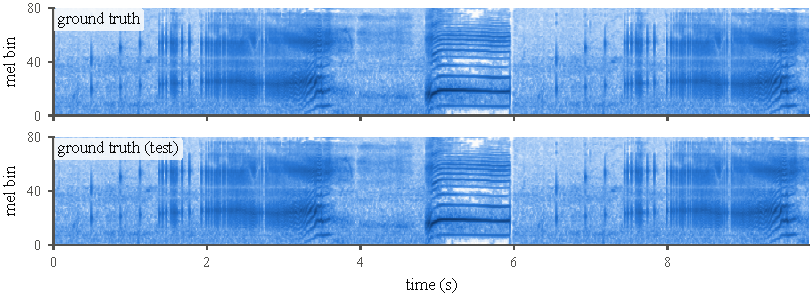
\includegraphics[width=\linewidth]{figures/vas_samples.pdf}
  \caption{One VAS test clip (the clip with the median $|$lag$|$ gain from best-of-4 re-ranking). Its $|$lag$|$ is 116\,ms for the single sample and 81\,ms for the best of four. VAS audio is dense, and timing differences of this size are hard to see in a spectrogram, which is why we report onset and envelope measures.}
  \label{fig:vas-samples}
\end{figure}


\end{document}
